%%\documentclass[a4paper,12pt,oneside]{llncs}
\documentclass[12pt,letterpaper]{article}
\usepackage[right=2cm,left=3cm,top=2cm,bottom=2cm,headsep=0cm]{geometry}

%%%%%%%%%%%%%%%%%%%%%%%%%%%%%%%%%%%%%%%%%%%%%%%%%%%%%%%%%%%
%% Juego de caracteres usado en el archivo fuente: UTF-8
\usepackage{ucs}
\usepackage[utf8x]{inputenc}

%%%%%%%%%%%%%%%%%%%%%%%%%%%%%%%%%%%%%%%%%%%%%%%%%%%%%%%%%%%
%% Juego de caracteres usado en la salida dvi
%% Otra posibilidad: \usepackage{t1enc}
\usepackage[T1]{fontenc}

%%%%%%%%%%%%%%%%%%%%%%%%%%%%%%%%%%%%%%%%%%%%%%%%%%%%%%%%%%%
%% Ajusta maergenes para a4
%\usepackage{a4wide}

%%%%%%%%%%%%%%%%%%%%%%%%%%%%%%%%%%%%%%%%%%%%%%%%%%%%%%%%%%%
%% Uso fuente postscript times, para que los ps y pdf queden y pequeños...
\usepackage{times}

%%%%%%%%%%%%%%%%%%%%%%%%%%%%%%%%%%%%%%%%%%%%%%%%%%%%%%%%%%%
%% Posibilidad de hipertexto (especialmente en pdf)
%\usepackage{hyperref}
\usepackage[bookmarks = true, colorlinks=true, linkcolor = black, citecolor = black, menucolor = black, urlcolor = black]{hyperref}

%%%%%%%%%%%%%%%%%%%%%%%%%%%%%%%%%%%%%%%%%%%%%%%%%%%%%%%%%%%
%% Graficos 
\usepackage{graphics,graphicx}

%%%%%%%%%%%%%%%%%%%%%%%%%%%%%%%%%%%%%%%%%%%%%%%%%%%%%%%%%%%
%% Ciertos caracteres "raros"...
\usepackage{latexsym}

%%%%%%%%%%%%%%%%%%%%%%%%%%%%%%%%%%%%%%%%%%%%%%%%%%%%%%%%%%%
%% Matematicas aun más fuertes (american math dociety)
\usepackage{amsmath}

%%%%%%%%%%%%%%%%%%%%%%%%%%%%%%%%%%%%%%%%%%%%%%%%%%%%%%%%%%%
\usepackage{multirow} % para las tablas
\usepackage[spanish,es-tabla]{babel}

%%%%%%%%%%%%%%%%%%%%%%%%%%%%%%%%%%%%%%%%%%%%%%%%%%%%%%%%%%%
%% Fuentes matematicas lo mas compatibles posibles con postscript (times)
%% (Esto no funciona para todos los simbolos pero reduce mucho el tamaño del
%% pdf si hay muchas matamaticas....
\usepackage{mathptm}

%%% VARIOS:
%\usepackage{slashbox}
\usepackage{verbatim}
\usepackage{array}
\usepackage{listings}
\usepackage{multirow}

%% MARCA DE AGUA
%% Este package de "draft copy" NO funciona con pdflatex
%%\usepackage{draftcopy}
%% Este package de "draft copy" SI funciona con pdflatex
%%%\usepackage{pdfdraftcopy}
%%%%%%%%%%%%%%%%%%%%%%%%%%%%%%%%%%%%%%%%%%%%%%%%%%%%%%%%%%%
%% Indenteacion en español...
\usepackage[spanish]{babel}
\usepackage{pdfpages}

\usepackage{listings}
% Para escribir código en C
% \begin{lstlisting}[language=C]
% #include <stdio.h>
% int main(int argc, char* argv[]) {
% puts("Hola mundo!");
% }
% \end{lstlisting}


\title{Tutorial de infraestructura de red Zybo}
\author{Jesús Rodríguez Heras}

\begin{document}
	
	\maketitle
	\begin{abstract} %Poner esto en todas las prácticas de PCTR
		\begin{center}
			En este documento se desarrolla la creación de la infraestructura de red física de cuatro placas Zybo, un ordenador y un switch.
		\end{center}
	\end{abstract}
	\thispagestyle{empty}
	\newpage
	
	\tableofcontents
	\newpage
	
	%%\listoftables
	%%\newpage
	
	%%\listoffigures
	%%\newpage
	
	%%%% REAL WORK BEGINS HERE:
	
	%%Configuracion del paquete listings
	\lstset{language=bash, numbers=left, numberstyle=\tiny, numbersep=10pt, firstnumber=1, stepnumber=1, basicstyle=\small\ttfamily, tabsize=1, extendedchars=true, inputencoding=latin1}


\section{Material necesario}
Para la creación de la infraestructura de red física de placas Zybo contaremos con el siguiente material:
\begin{itemize}
	\item 4 placas Zybo Zynq-7000.
	\item Un ordenador con sistema operativo Linux (Debian 9 Stretch) y Windows 7.
	\item Un switch tp-link modelo TL-SG1024D.
\end{itemize}


\subsection{Placas Zybo Zynq-7000}
\begin{figure}[h]
	\centering
	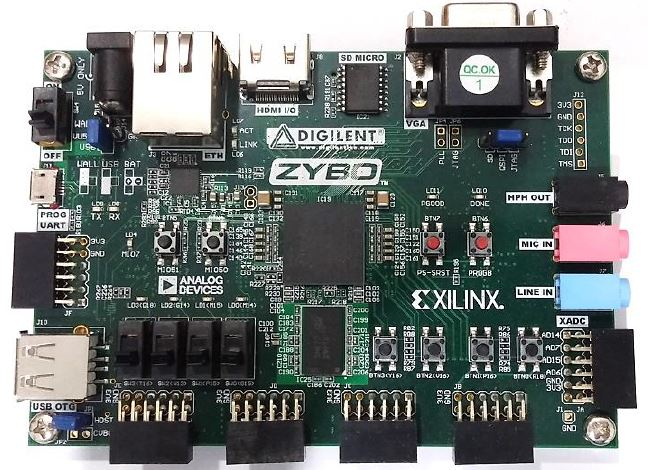
\includegraphics[scale=0.5]{zybo.jpg}
\end{figure}
Para este proyecto necesitaremos poder programar la FPGA integrada en la placa desde la tarjeta SD de memoria. Para ello, tendremos que cambiar el jumper JP5 (situado arriba a la derecha) en los pines situados más a la izquierda. Dicho jumper está identificado con el número 21 en la siguiente página.

%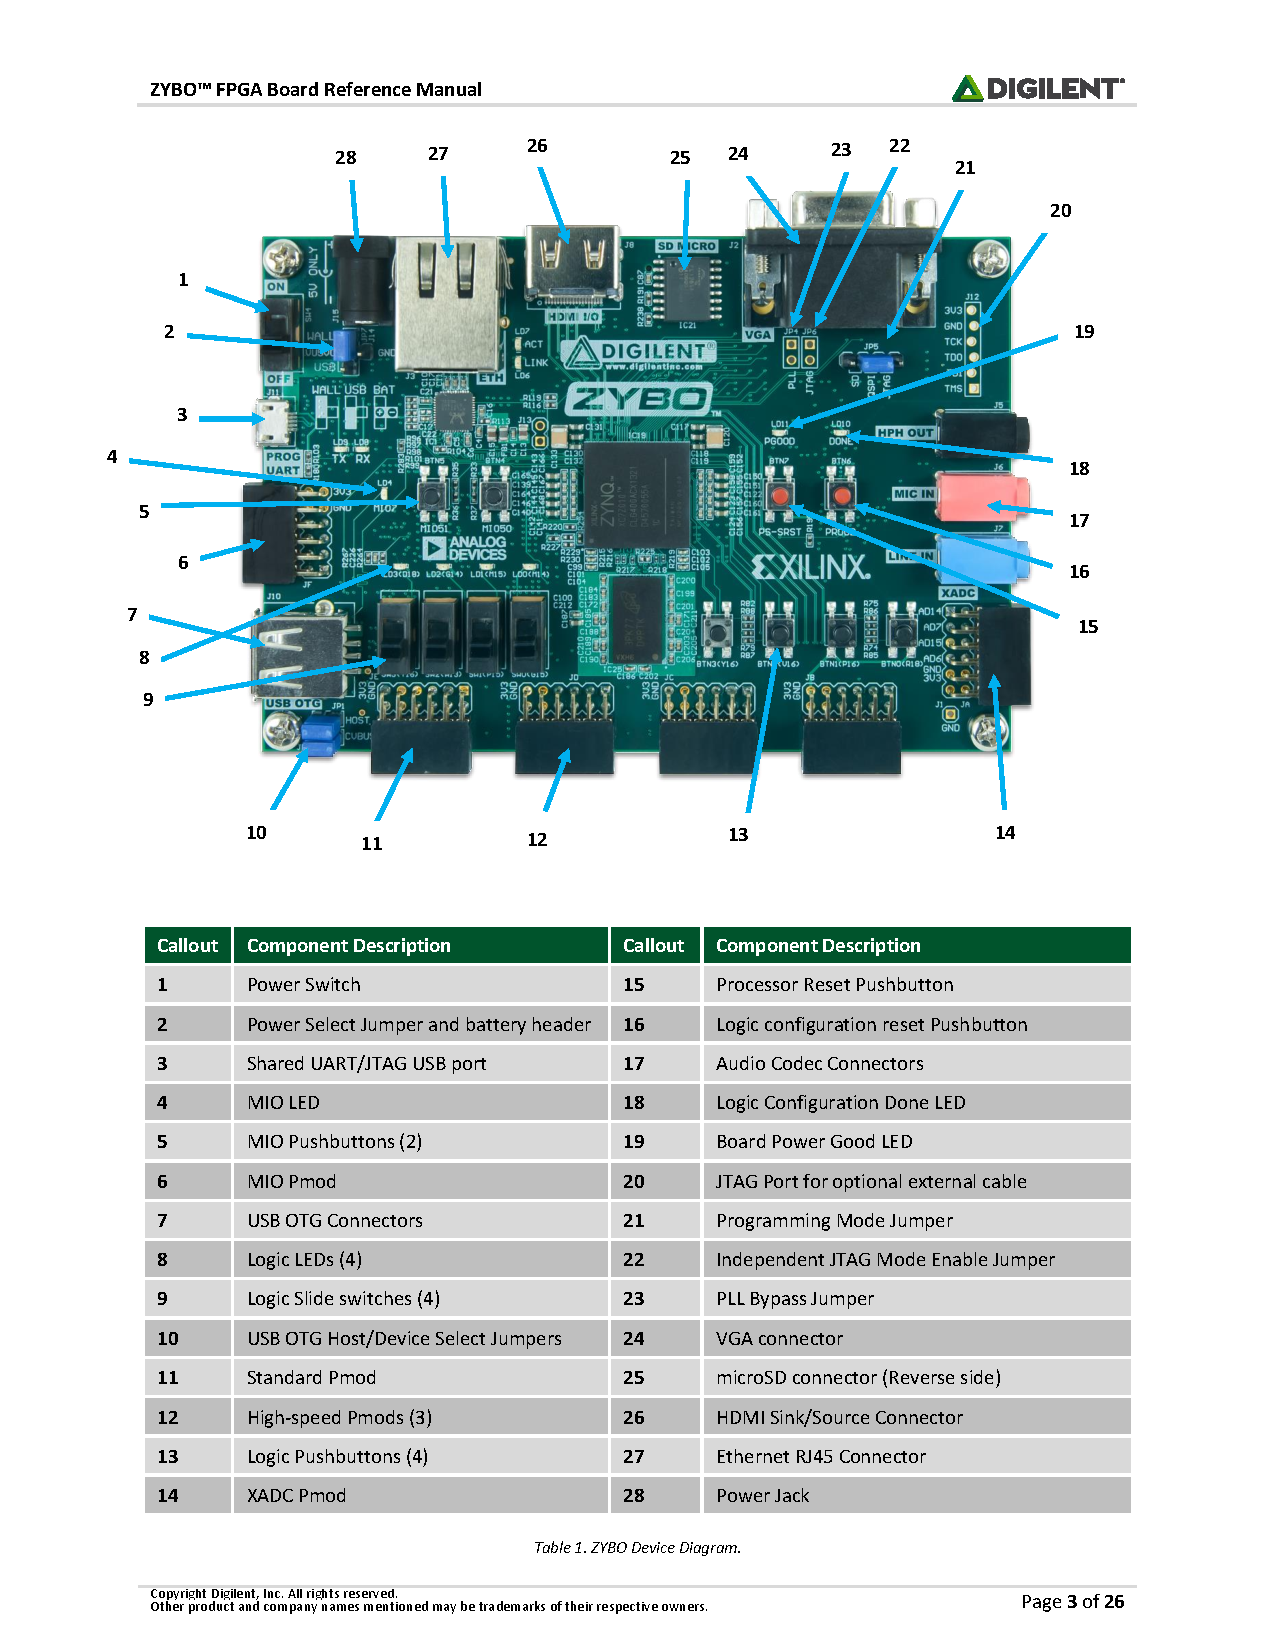
\includepdf[pages=-]{Datasheet.pdf}
%\begin{figure}[h]
%	\centering
%	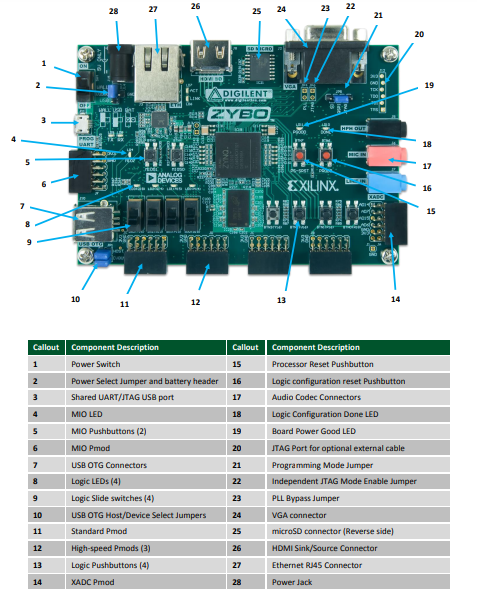
\includegraphics[scale=1]{Datasheet.png}
%\end{figure}

\newpage

\subsection{Ordenador}
El ordenador usado en el proyecto tendrá dos sistemas operativos.
\begin{itemize}
	\item \textbf{Debian 9 Stretch:} En este sistema operativo se realizará la compilación del sistema operativo Linux de las tarjetas Zybo y la programación del bitstream con el software de Vivado. El usuario será \texttt{zybo} y la contraseña de acceso, será \texttt{zybomonitor}. Asimismo, la contraseña de superusuario también será \texttt{zybomonitor}.
	\item \textbf{Windows 7:} También tendrá la capacidad de programar la FPGA de la tarjeta.
\end{itemize}

\subsection{Switch}
El switch usado en este proyecto es el tp-link TL-SG1024D que cuenta con 24 puertos con tecnología Gigabit y conectores RJ-45.


\section{Pasos para el montaje de la infraestructura}
Llegados a este paso suponemos que las tarjetas ya tienen su sistema operativo instalado, pueden arrancar e iniciar sesión y se le ha asignado su dirección IP correspondiente.

Las tarjetas estarán identificadas como ZyboX (siendo ``X'' un número entre 1 y 4) y el ordenador se identificará como ``Monitor''.

Los dispositivos tendrán la siguiente configuración de red:
\begin{table}[h]
	\centering
	\begin{tabular}{|c|c|}
		\hline
		\textbf{Dispositivo} & \textbf{Dirección IP} \\ \hline
		Monitor & 192.168.1.1 \\ \hline
		Zybo1 & 192.168.1.2 \\ \hline
		Zybo2 & 192.168.1.3 \\ \hline
		Zybo3 & 192.168.1.4 \\ \hline
		Zybo4 & 192.168.1.5 \\ \hline
	\end{tabular}
\end{table}

Una vez tengamos los dispositivos identificados tenemos que conectarlos al switch\footnote{Podemos conectar los dispositivos al puerto del switch que queramos debido a que se encargará de ir rellenando su tabla CAM con las direcciones de los dispositivos que tiene conectados.}.

\end{document}